\chapter{Dasar Teori}
\label{chap:dasarteori}

\section{\textit{Mobile Cloud Computing}}
\label{sec:mobilecloudcomputing}

Pada sub-bab ini akan dibahas mengenai pengertian dan arsitektur \textit{Mobile Cloud Computing}.

\subsection{Pengertian \textit{Cloud Computing}}
\label{subsec:pengertiancloud}
\hspace{0,5cm} \textit{Cloud Computing} adalah gabungan pemanfaatan komputer dan pengembangan berbasis internet. \textit{Cloud Computing} menawarkan kemudahan layanan terkait informasi tanpa pengguna mengetahui apa yang ada di dalamnya.

\subsection{Manfaat \textit{Cloud Computing}}
\label{subsec:pengertianmanfaatcloud}
\begin{itemize}
	\item Skalabilitas, yaitu memudahkan dalam perluasan penambahan kapasitas.
	\item Aksesibilitas, yaitu memudahkan dalam pengaksesan dimanapun dan kapanpun.
	\item Keamanan
	\item Kreasi
	\item Kecemasan
\end{itemize}

\subsection{Layanan \textit{Cloud Computing}}
\label{subsec:pengertianlayanancloud}
\begin{itemize}
	\item Infrastructure as a Service (IaaS)\\
	merupakan layanan \textit{Cloud Computing} yang menyediakan infrastruktur IT berupa CPU, RAM, storage, bandwith dan konfigurasi lain.
	\begin{figure}[h]
		\centering
			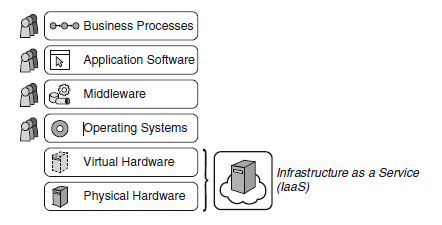
\includegraphics{Gambar/iaas-infrastruktur}
		\caption{Infrastruktur as a Service Stack}
		\label{fig:iaas-infrastruktur}
	\end{figure}
	\item Platform as a Service (PaaS)\\
	merupakan layanan yang menyediakan computing platform. Biasanya sudah terdapat sistem operasi, database, web server dan framework aplikasi agar dapat menjalankan aplikasi yang telah dibuat.
	\begin{figure}[h]
		\centering
			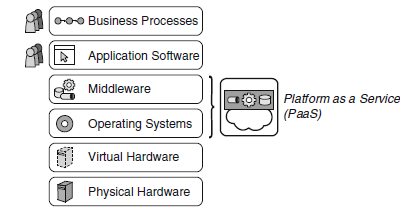
\includegraphics{Gambar/paas-infrastruktur}
		\caption{Infrastruktur as a Service Stack}
		\label{fig:iaas-infrastruktur}
	\end{figure}
	\item Software as a Service (SaaS)\\
	merupakan layanan komputasi awan dimana kita bisa langsung menggunakan aplikasi yang telah disediakan.
	\begin{figure}[h]
		\centering
			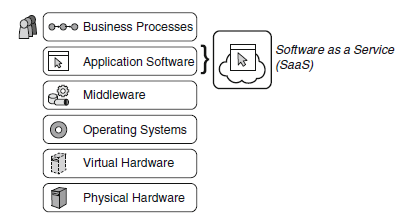
\includegraphics{Gambar/saas-infrastruktur}
		\caption{Infrastruktur as a Service Stack}
		\label{fig:iaas-infrastruktur}
	\end{figure}
\end{itemize}

\section{Android}
\label{sec:android}

Pada sub-bab ini akan dibahas mengenai pengertian dan arsitektur Android.

\subsection{Pengertian Android}
\label{subsec:pengertianandroid}

Android merupakan sistem operasi buatan Google untuk \textit{mobile device}. Saat penelitian ini dilakukan Sistem operasi Android menjadi yang paling populer dan sudah digunakan oleh lebih dari 100 juta pengguna di seluruh dunia. Kesuksesan Android tidak lepas dari basis \textit{open-source} yang memungkinkan pembuatan varian kustom dari Android.
%http://developer.android.com/index.html
%about -> http://developer.android.com/about/index.html

\subsection{Arsitektur Android}
\label{subsec:arsitektur}

Secara umum arsitektur Android dibagi menjadi empat lapisan. Lapisan arsitektur Android dapat dilihat pada Gambar~\ref{fig:arsitektur_android}\footnote{http://elinux.org/Android\_Architecture}. Berikut ini adalah penjelasan mengenai empat lapisan pada arsitektur Android.

\begin{enumerate}
\item \textit{Applications} merupakan lapisan teratas yang berhubungan dengan pengguna.
\item \textit{Applications Framework} merupakan lapisan yang digunakan oleh para penggembang aplikasi. Pada lapisan ini terdapat \textit{framework} yang dapat digunakan orang para pengembang aplikasi. %Jelasin apa itu framework
\item \textit{Libraries} merupakan kumpulan-kumpulan fungsi yang disediakan oleh Android.
\item \textit{Linux Kernel} merupakan kumpulan-kumpulan fungsi yang berhubungan langsung dengan perangkat keras.
\end{enumerate}

\begin{figure}
\centering
\resizebox{\textwidth}{!}{
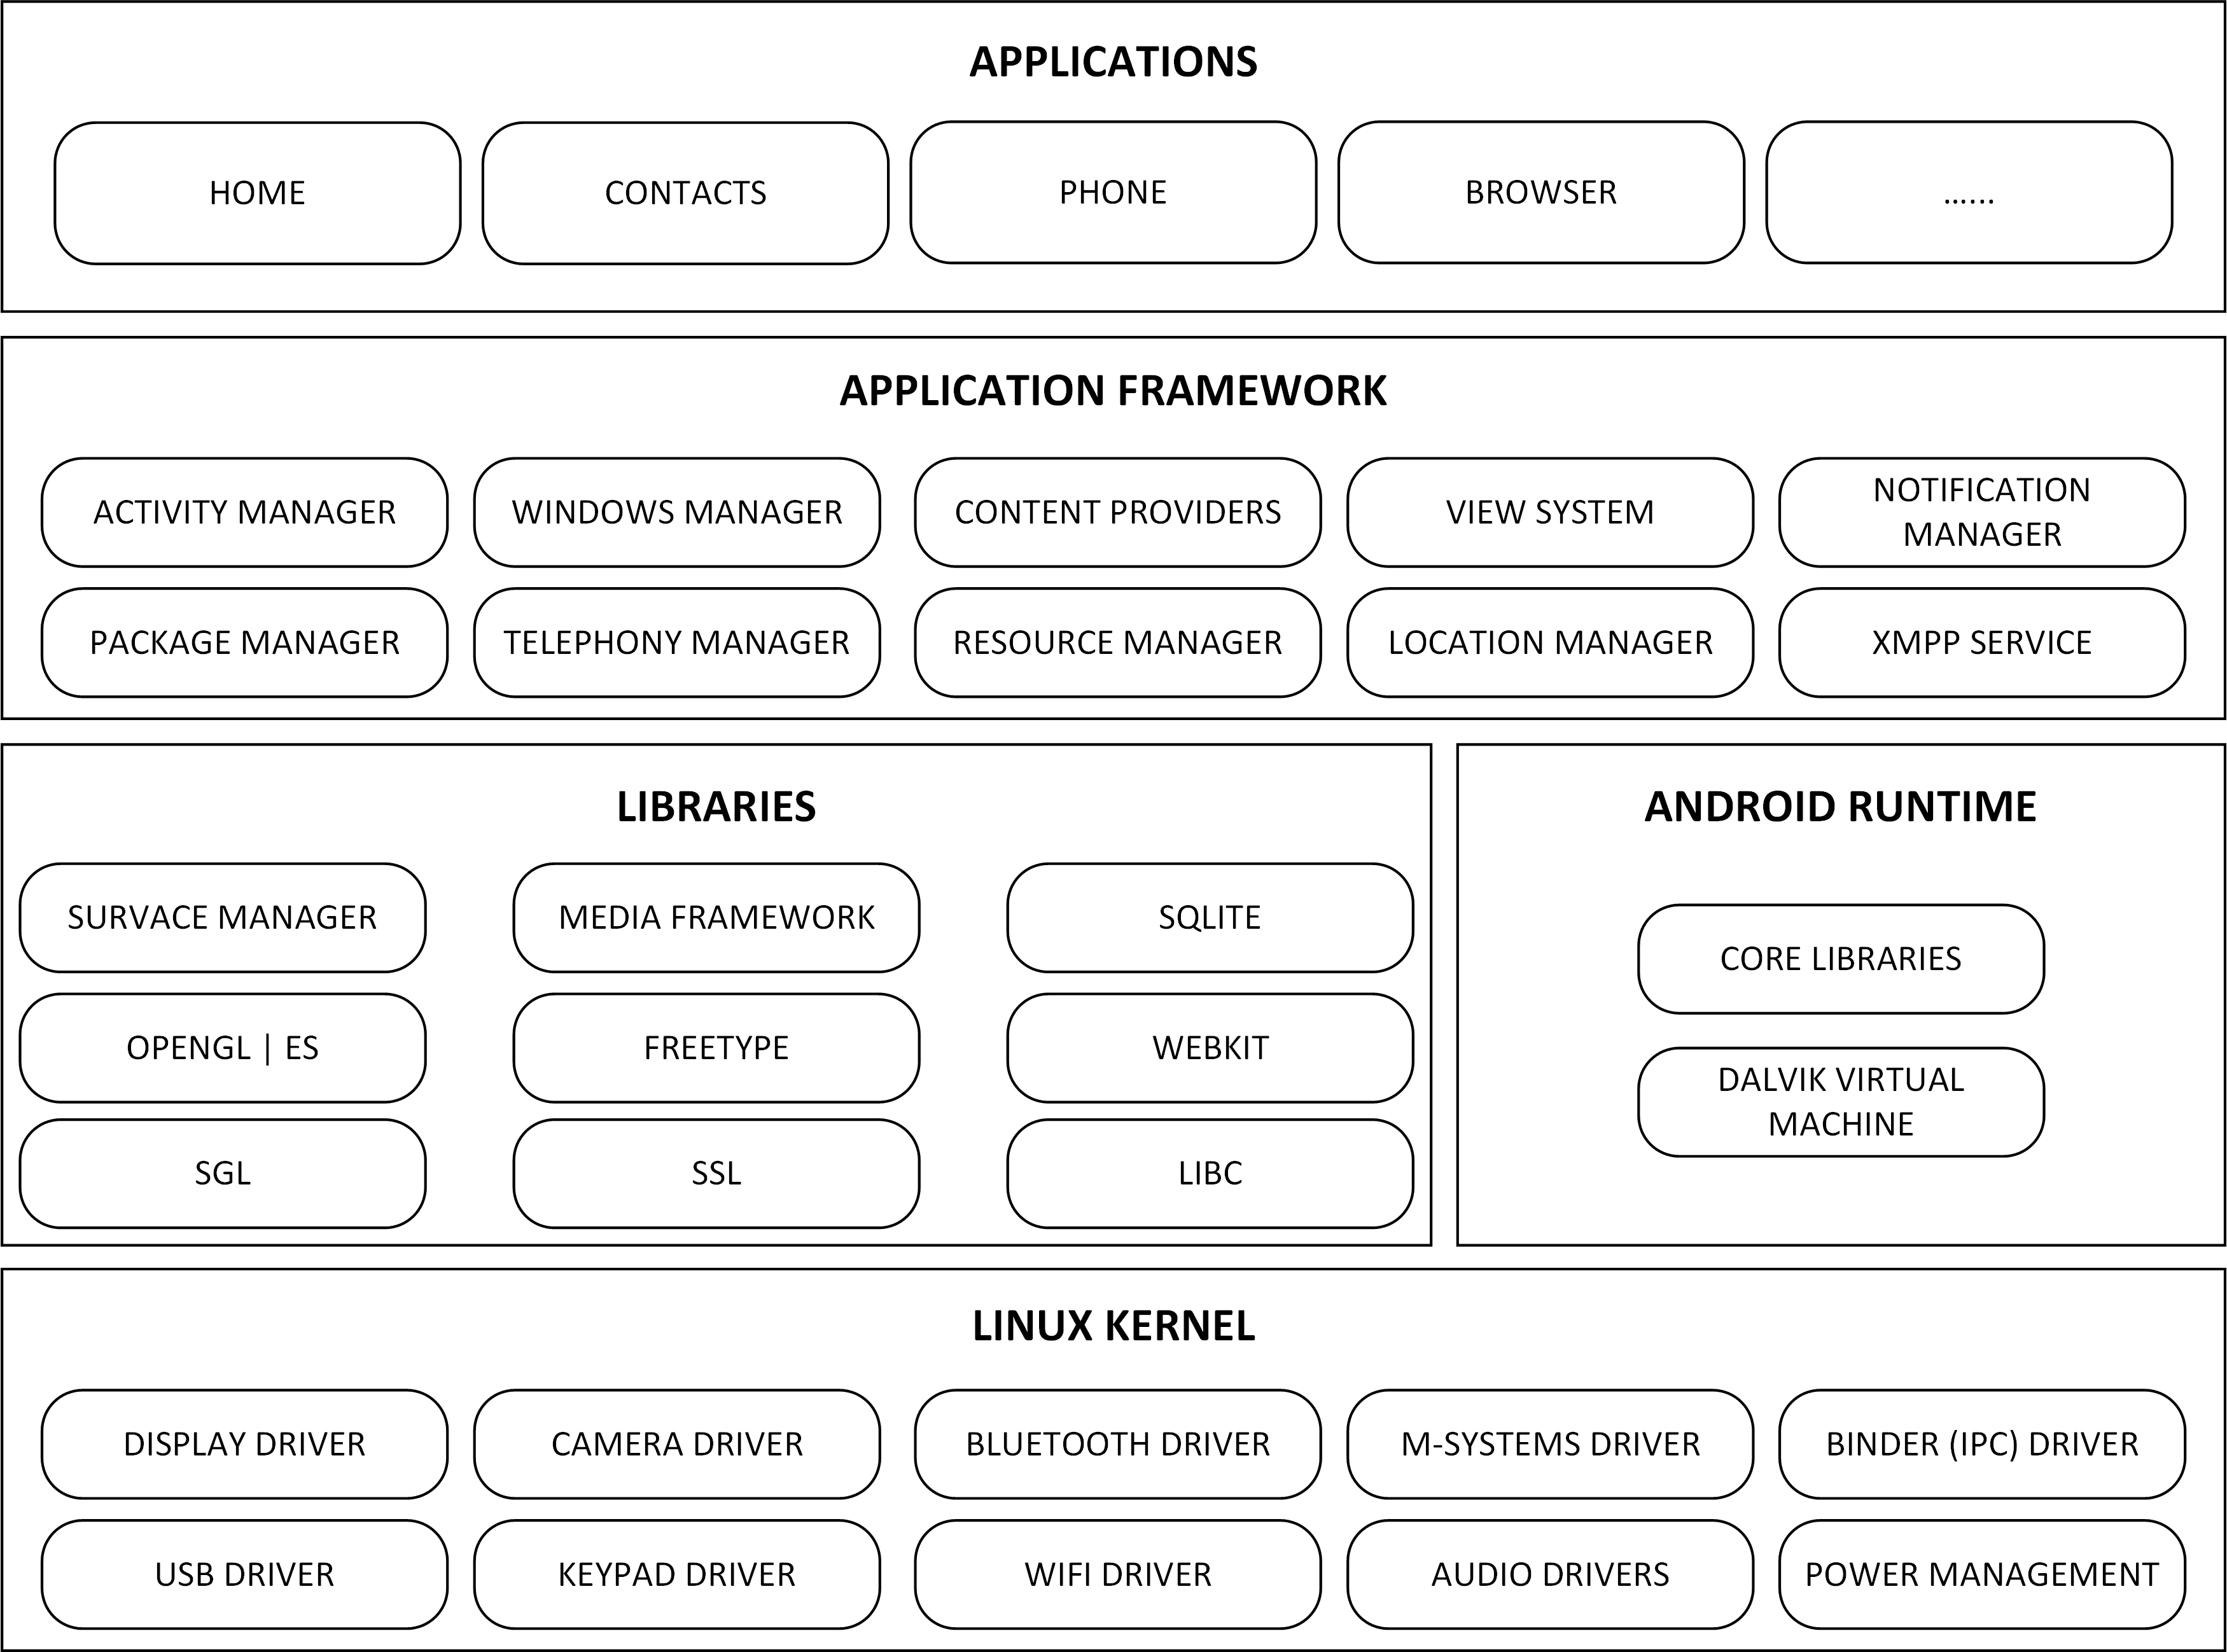
\includegraphics{Gambar/Android-system-architecture}
}
\caption[Arsitektur Android]{Arsitektur Android} 
\label{fig:arsitektur_android}
\end{figure}

\subsection{\textit{Life Cycle}}
\label{subsec:lifecycle}

Aplikasi yang berjalan pada Android memiliki \textit{lifecycle} sesuai dengan rancangan sistem operasi Anrdroid. \textit{Lifecycle} aplikasi pada Android dapat dilihat pada gambar \ref{fig:dasar_lifecycle_android}.

\begin{figure}
\centering
\resizebox{\textwidth}{!}{
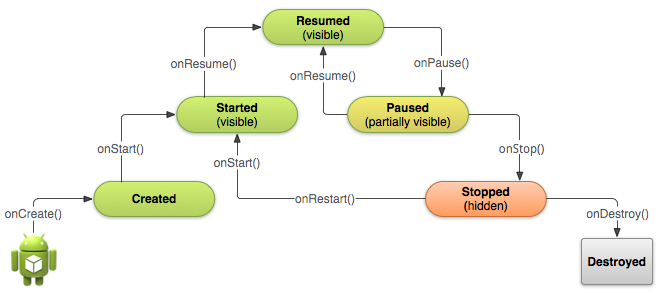
\includegraphics{Gambar/basic-lifecycle}
}
\caption[Dasar \textit{lifecycle} Android]{Dasar \textit{lifecycle} Android} 
\label{fig:dasar_lifecycle_android}
\end{figure}

\section{Phonegap}
\label{sec:phonegap}

\subsection{Pengertian Phonegap}
\label{sec:pengertianphonegap}

Phonegap merupakan suatu \textit{framework} yang digunakan untuk mengembangkan aplikasi pada perangkat mobile. Phonegap memungkinkan aplikasi dibangun di atas Javascript, HTML5, dan CSS3\footnote{Jose Fermoso (April 5, 2009). "PhoneGap Seeks to Bridge the Gap Between Mobile App Platforms"}.

\subsection{Arsitektur Phonegap}
\label{sec:arsitekturphoengap}

Phonegap menggunakan HTML\ref{subsec:html} dan CSS\ref{subsec:css} untuk me-\textit{render} aplikasi dan Javascript\ref{subsec:javascript} digunakan untuk menjalankan logika dari aplikasi yang dibuat. Phonegap membangun API yang dapat digunakan oleh pengembang aplikasi di atas OS \textit{mobile device}. Arsitektur Phonegap dapat dilihat pada Gambar~\ref{fig:arsitektur_phonegap} 

\begin{figure}
\centering
\resizebox{\textwidth}{!}{
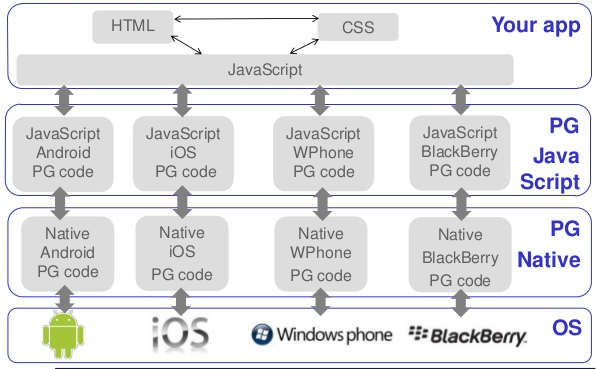
\includegraphics{Gambar/phonegap-architecture}
}
\caption[Arsitektur Phonegap]{Arsitektur Phonegap} 
\label{fig:arsitektur_phonegap}
\end{figure}

\subsection{HTML}
\label{subsec:html}

HTML merupakan suatu bahasa standar yang digunakan untuk membuat halaman situs\footnote{http://www.merriam-webster.com/dictionary/hypertext markup language}.

\subsection{CSS}
\label{subsec:css}

CSS merupakan suatu bahasa yang digunakan untuk menformat tampilan suatu dokumen.

\subsection{Javascript}
\label{subsec:javascript}

Javascript merupakan bahasa pemograman yang pada umumnya digunakan pada \textit{web browser}.

\section{Hadoop and \textit{Ecosystem}}
\label{sec:hadoopandecosystem}

\subsection{Hadoop}
\label{subsec:hadoop}

Hadoop merupakan sebuah \textit{platform} yang menyediakan pemyimpanan data terdistribusi dan kemampuan komputasi. Kemampuan komputasi pada Hadoop merupakan \textit{distributed master-slave architeture} yang terdiri dari Hadoop Distributed File System (HDFS)\ref{subsec:hdfs} untuk penyimpanan data dan MapReduce \ref{subsec:mapreduce}. Arsitektur Hadoop dapat dilihat pada Gambar \ref{fig:arsitektur_hadoop}\cite{holmes2012hadoop}.

\begin{figure}
\centering
\resizebox{\textwidth}{!}{
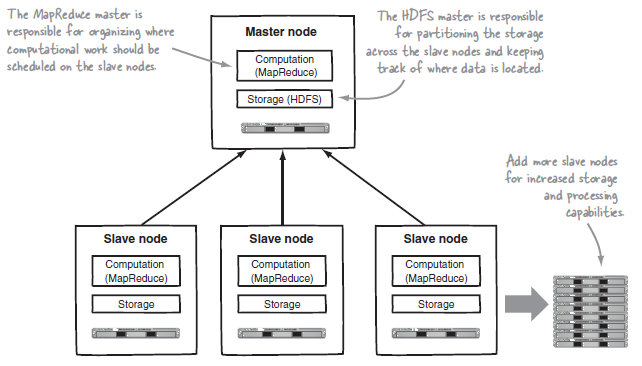
\includegraphics{Gambar/high-level-hadoop-architecture}
}
\caption[Arsitektur Hadoop]{Arsitektur Hadoop} 
\label{fig:arsitektur_hadoop}
\end{figure}

\subsection{HDFS}
\label{subsec:hdfs}

HDFS adalah komponen penyimpanan data dari Hadoop yang merupakan sistem penyimpanan data terdistribusi. Arsitektur HDFS dapat dilihat pada Gambar \ref{fig:arsitektur_hdfs}

\begin{figure}
\centering
\resizebox{\textwidth}{!}{
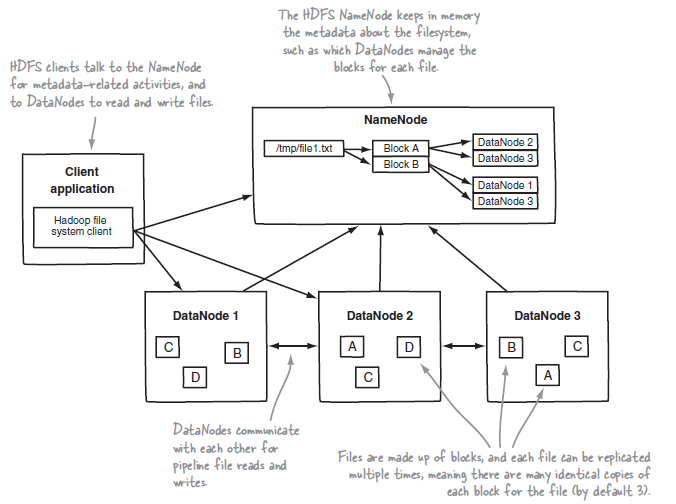
\includegraphics{Gambar/arsitektur-hdfs}
}
\caption[Arsitektur HDFS]{Arsitektur HDFS} 
\label{fig:arsitektur_hdfs}
\end{figure}

\subsection{MapReduce}
\label{subsec:mapreduce}

\hspace{0,5cm}MapReduce merupakan \textit{batch-based}, komputasi terdistribusi \textit{framework} yang memungkinkan komputasi paralel terhadap data yang cukup besar. MapReduce menyederhanakan pemrosesan paralel oleh abstraksi kerja yang komplek. Dengan abstraksi ini, MapReduce memungkinkan \textit{programmer} untuk berfokus pada kebutuhan bisnis dibandingkan memikirkan sistem distribusinya.

\subsection{HBase}
\label{subsec:hbase}

HBase merupakan \textit{real-time, column-oriented} basis data yang dapat diintergrasi kedalam HDFS melalu MapReduce.

%Apa itu Hbase?

\subsection{Trafodion}
\label{subsec:trafodian}

Trafodion merupakan \textit{open source project} yang disponsor oleh HP. Trafodion juga diinkubasi di HP Labs dan HP-IT yang digunakan untuk mengembangkan SQL-on-Hadoop berskala \textit{enterprise} terhadap data yang besar\footnote{https://wiki.trafodion.org/wiki/index.php/Main\_Page}. 

\section{Webservice and RESTful}
\label{sec:webserviceansrestful}

Pada sub-bab ini akan dibahas mengenai Webservice dan RESTful.

\subsection{Webservice}
\label{subsec:webservice}

Webservice merupakan suatu sistem yang menyediakan fungsi-fungsi dari suatu perangkat lunak diatas internet melalui \textit{web}.

\subsection{RESTful}
\label{subsec:restful}

\textit{Representational State Transfer}(REST) merupakan gaya arsitektur suatu perangkat lunak yang terdiri dari pedoman dan praktek terbaik untuk membuat suatu \textit{webservice}\ref{subsec:webservice} yang \textit{scalable}\footnote{Fielding, R. T.; Taylor, R. N. (2000). "Principled design of the modern Web architecture". pp. 407\-416. doi:10.1145/337180.337228}

\section{Google Open Authentication (OAuth)}
\label{sec:googleopenauthentication}

Pada sub-bab ini akan dibahas mengenai OAuth dan Google Oauth.

\subsection{Open Authentication (OAuth)}
\label{subsec:oauth}

\hspace{0,5cm}OAuth merupakan standar terbuka untuk autentikasi. Oauth menyediakan akses yang aman kepada klien untuk mengakses \textit{server}. Hal ini menjadikan \textit{server} dapat diakses oleh \textit{third-party}. Desain OAuth diatas HTTP. Prinsip OAuth pada dasarnya menyediakan akses token kepada klien/pengguna akhir sehingga dapat digunakan untuk bertransaksi dengan \textit{server}\footnote{http://tools.ietf.org/html/rfc6749}.

\subsection{Google \textit{OAuth}}
\label{subsec:googleip}

\hspace{0,5cm}Google OAuth merupakan protokol OAuth yang digunakan oleh google untuk memberikan akses kepada \textit{third-party} untuk mengakses API mereka. Skema untuk mengakses Google OAuth dapat dilihat pada Gambar~\ref{fig:google_oauth}.

\begin{figure}
\centering
\resizebox{\textwidth}{!}{
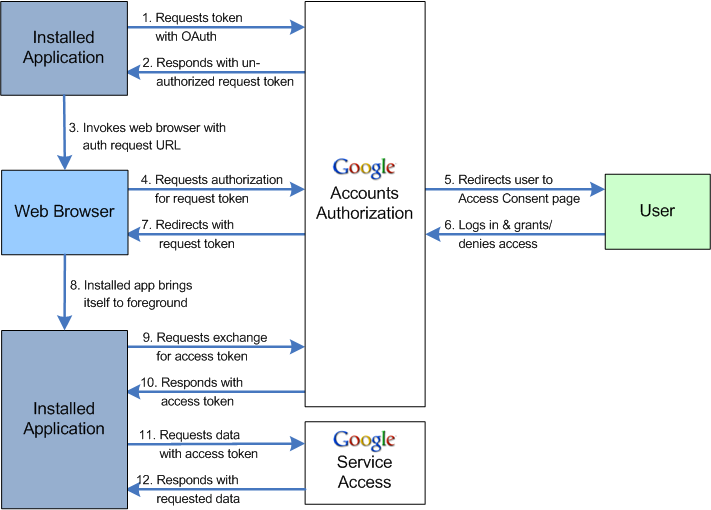
\includegraphics{Gambar/google-oauth}
}
\caption[Google OAuth]{Google OAuth} 
\label{fig:google_oauth}
\end{figure}

\subsection{Google \textit{Identity Platform}}
\label{subsec:googleidentityplatform}
\hspace{0,5cm} Merupakan layanan dari Google yang memberikan kemudahan dan keamanan  untuk masuk ke situs dan aplikasi dengan mudah. Untuk memanfaatkan layanan dibutuhkan pemanfaatan API di situs maupun aplikasi. Solusi layanan yang dapat digunakan untuk Android, iOS, dan situs adalah Google Sign-In. Berikut kegunaan dari Google Sign-In.
\begin{itemize}
	\item Mendapatkan pengguna untuk mengakses aplikasi dengan cepat dan aman dengan pengembangan yang sedikit. 
	\item Pengguna cukup \textit{sign-in} sekali dan di \textit{authenticated} di semua perangkat mereka.
	\item Layanan Google yang terintegrasi
	\item Memungkinkan instalasi dari aplikasi Android ketika pengguna masuk ke situs
\end{itemize}
   
%API = https://developers.google.com/identity/sign-in/web/sign-in